\documentclass[9pt,twocolumn,twoside]{opticajnl}
\journal{opticajournal} % use for journal or Optica Open submissions

% See template introduction for guidance on setting shortarticle option
\setboolean{shortarticle}{true}
% true = letter/tutorial
% false = research/review article

% ONLY applicable for journal submission shortarticle types:
% When \setboolean{shortarticle}{true}
% then \setboolean{memo}{true} will print "Memorandum" on title page header
% Otherwise header will remain as "Letter"
% \setboolean{memo}{true}


\usepackage{lineno}
\usepackage{verbatim}

\linenumbers % Turn off line numbering for Optica Open preprint submissions.

\title{Análisis descriptivo de conjunto de datos}

\author[1,2,3]{Luis Ardévol Mesa}


\begin{abstract}
Se analizará un conjunto de datos de temperatura media y precipitacion acumulada sobre las Islas Canarias desde 1980 hasta 2099. Con la temperatura, se pretende mostrar el aumento de la temperatura media en ese rango de tiempo. Con la precipitación, se pretende mostrar la disminución de la precipitación acumulada en el mismo rango de tiempo. 
\end{abstract}

\setboolean{displaycopyright}{false} % Do not include copyright or licensing information in submission.

\begin{document}

\maketitle

\section{Descripción y objetivos}

El conjunto de datos es el resultado de mi Trabajo de Fin de Grado, \textit{Climate regionalisation through machine learning techniques}. El objetivo del mismo era emular los resultados de regionalizaciones dinámicas realizadas por el GOTA de la Universidad de La Laguna usando el modelo WRF. \\

Primero, demos un poco de contexto a estos datos: se trata de predicciones de una regionalización estadística que se sirve de dos redes neuronales convolucionales entrenadas con datos de reanálisis de ERA-5, usando 5 predictores estándar propuesto por la acción VALUE COST. Estos se extienden sobre una región $(22, 40)^\circ$ N en latitud y $(-32, 0)^\circ$ E en longitud, y abarcan desde 1982 hasta 2010. El resultado, es decir, los datos que se van a usar, son predicciones de temperatura media y precipitacion acumulada sobre una región $(27.5, 29.3)^\circ$ N en latitud y $(-18.2, -13.4)^\circ$ E en longitud, lo que abarca las Islas Canarias (solo considerando los puntos de tierra, luego se remapean al grid completo para mostrar visualmente el océano). Las predicciones tienen un valor diario para ambas variables en los periodos de tiempo desde 1980 hasta 2009, 2030-2059 y 2070-2099. Estos resultados se obtienen usando como \textit{samples} datos y proyecciones de 3 modelos climáticos globales (GCMs), que proporcionan los 5 predictores mencionados anteriormente. Las proyecciones empleadas consideran el escenario de emisiones RCP 8.5. Los resultados disponible presentan una dimensión temporal y otra espacial. Tras el remapeo comentado en el origen de los datos, la dimensión espacial se aumenta a un grid, dando así una tercera dimensión a estos arrays. Se muestran todos en el siguiente \texttt{\href{https://drive.google.com/drive/folders/1iwTRm0Ibb-NRyxuiQCVuFF2_RFj2Wlel?usp=share_link}{enlace}}. \\

El objetivo de este análisis es mostrar el aumento en la temperatura media, de aquí a final de siglo, que sería de esperar debido al escenario de emisiones considerado en las proyecciones (debería estar entre $2.6^\circ$ y $4.8^\circ$). De forma similar, se pretende mostrar la disminución de la precipitación acumulada en aproximadamente un $20\%$, de aquí a final de siglo, esperada en zonas como Canarias según el escenario escogido. 


\section{Datos y variables de interés}

Debido a la gran cantidad de datos disponibles, se tomará directamente un subconjunto de los mismos. Como criterio de elección, se hará uso de los datos que mejor emularon las regionalizaciones dinámicas: para temperatura, se usarán los datos obtenidos con el modelo climático global GFDL-ESM2M, mientras que para precipitaciones se escogen los obtenidos con el modelo IPSL-CM5A-MR. Se tomarán los datos de los tres periodos temporales: 1980-2009, 2030-2059 y 2070-2099 (con valores diarios, excepto datos corruptos). Para el análisis, se cargarán únicamente los datos de puntos de tierra (1059) y, únicamente para la visualización, se cargarán los mismos datos remapeados al grid completo ($68 \times 158$). \\

Las variables bajo estudio serán la temperatura media y la precipitación acumulada. En este caso, ambas son variables cuantitativas continuas: la temperatura puede tomar cualquier valor dentro de su rango teórico (del cero absoluto a la temperatura de Planck), mientras que la precipitación acumulada puede tomar cualquier valor no negativo. 

\section{Resumen numérico}

Se disponen de datos temporales y espaciales. Una opción sería hacer una media en la dimensión espacial para estudiar la variación de las variables en Canarias con el tiempo durante los periodos de estudio. Al tener periodos de tiempo tan amplios, resulta también interesente para disciplinas relacionadas con el clima hacer un análisis de la variación de las variables espacialmente durante cada uno de los periodos. 

\subsection{Asimetría}

Típicamente (aunque depende del caso no es correcto), la temperatura media se asocia a una distribución gaussiana. En este caso, la precipitación se obtuvo minimizando una distribución Bernouilli-Gamma, por lo que solo se verá la asimetría de la variable temperatura. Para estos datos, se tiene la asimetría de la distribución espacial (un valor para cada día) y la temporal (un valor para cada punto de tierra), pudiéndose estudiar por separado; se verá el número de valores que caen en ciertos rangos para sacar conclusiones (tablas \ref{tb:1} y \ref{tb:2}). \\

En el caso de la distribución espacial, se observa una alta asimetría en los tres periodos, con gran cantidad de ellos siendo menores que $-1$. Esto indica que el grueso de los datos se desvía hacia valores altos, generando una cola larga en el rango de las x negativas. En el caso de la distribución temporal, se mantiene cierta simetría, con una mayor cantidad de valores en el rango $[0, 0.5)$. 

\begin{table}[h]
\centering
\resizebox{0.33\textwidth}{!}{
\begin{tabular}{cccc}
\hline
\textbf{Asimetría} & \textbf{1980-2009} & \textbf{2030-2059} & \textbf{2070-2099} \\ \hline
< -1 & 6511 & 6595 & 5764 \\ \hline
[-1, -0.5) & 2460 & 2223 & 2155 \\ \hline
[-0.5, 0) & 828 & 969 & 1183 \\ \hline
0 & 0 & 0 & 0 \\ \hline
(0, 0.5] & 667 & 782 & 1326 \\ \hline
(0.5, 1] & 105 & 245 & 458 \\ \hline
> 1 & 0 & 0 & 0 \\ \hline
\end{tabular}
}
\caption{Salida de código: número de puntos con cada valor de asimetría espacial de la temperatura.}
\label{tb:1}
\end{table}

\begin{table}[H]
\centering
\resizebox{0.33\textwidth}{!}{
\begin{tabular}{cccc}
\hline
\textbf{Asimetría} & \textbf{1980-2009} & \textbf{2030-2059} & \textbf{2070-2099} \\ \hline
< -1 & 0 & 0 & 0 \\ \hline
[-1, -0.5) & 0 & 0 & 0 \\ \hline
[-0.5, 0) & 0 & 0 & 0 \\ \hline
0 & 0 & 0 & 0 \\ \hline
(0, 0.5] & 599 & 648 & 708 \\ \hline
(0.5, 1] & 460 & 411 & 351 \\ \hline
> 1 & 0 & 0 & 0 \\ \hline
\end{tabular}
}
\caption{Salida de código: número de puntos con cada valor de asimetría temporal de la temperatura.}
\label{tb:2}
\end{table}

El motivo de esta gran discrepancia entre las distribuciones espacial y temporal se debe al teorema del límite central. Si bien las distribuciones no tienen por qué ser guassianas, al estudiar la asimetria temporal se han promediado más de 10000 valores para dejar los 1059 puntos de tierra, mientras que en la distribución espacial se han promediado 1059 valores para dejar un solo punto de tierra. Por tanto, que la distribución temporal se asemeje más a una gaussiana es consecuencia directa de este teorema.

\begin{table}[h]
\centering
\resizebox{0.4\textwidth}{!}{
\begin{tabular}{cccc}
\hline
\textbf{Medida} & \textbf{1980-2009} & \textbf{2030-2059} & \textbf{2070-2099} \\ \hline
Media$_1$ $[^\circ C]$ & $16.022$ & $17.537$ & $19.010$ \\ \hline
Media$_2$ $[^\circ C]$& $16.022$ & $17.537$ & $19.010$ \\ \hline
Mediana$_1$ $[^\circ C]$ & $16.484$ & $17.912$ & $19.283$ \\ \hline
Mediana$_2$ $[^\circ C]$ & $15.365$ & $16.789$ & $18.194$ \\ \hline
$\sigma_1$ $[^\circ C]$ & $2.631$ & $2.530$ & $2.470$ \\ \hline
$\sigma_2$ $[^\circ C]$ & $3.617$ & $3.791$ & $3.988$ \\ \hline
Media$_1$ [mm/día] & $0.232$ & $0.171$ & $0.141$ \\ \hline
Media$_2$ [mm/día] & $0.232$ & $0.171$ & $0.141$ \\ \hline
Mediana$_1$ [mm/día] & $0.110$ & $0.064$ & $0.033$ \\ \hline
Mediana$_2$ [mm/día] & $0.002$ & $0.007$ & $0.019$ \\ \hline
$\sigma_1$ [mm/día] & $0.429$ & $0.394$ & $0.405$ \\ \hline
$\sigma_2$ [mm/día] & $1.259$ & $1.018$ & $0.687$ \\ \hline
\end{tabular}
}
\caption{Salida de código: medidas de posición y dispersión en los tres periodos. $[^\circ C]$ para temperatura y [mm/día] para precipitación. Con subíndice 1 los calculados como promedio de las medidas en la dimensión espacial y con subíndice 2 los calculados como promedio de las medidas en la dimensión temporal.}
\label{tb:4}
\end{table}


\subsection{Posición y dispersión}

Se calculará la media y mediana de los datos, para verificar si son próximas, y además se calculará la desviación estándar para dar cuenta de la dispersión de los datos en las unidades de los mismos. De nuevo surge el problema de la cantidad de datos al promediar en una dimensión, así que se muestran los resultados medios de calcular estas medidas en una dimensión concreta. \\

Se ven los resultados en la tabla \ref{tb:4}. En el caso de los promedios de las medidas en la dimensión espacial, se tiene un valor respresentativo de la serie temporal, perdiendo detalles de la variabilidad espacial en cada instante. En el otro caso, se tienen valores representativos de todo el espacio, perdiendo detalles de la variabilidad temporal. En términos absolutos la desviación estándar de estos últimos es mayor, mientras que la mediana se situa por debajo de la media, comportamiento contrario al de los promedios de las medidas en la dimensión temporal. En ambos casos se puede ver claramente el aumento de la temperatura y el descenso de las precipitaciones de aquí a final de siglo.


\section{Resumen gráfico}

\subsection{Distribución temporal}

Para visualizar la distribución temporal de las variables, se mostrará la variabilidad temporal de cada año con un gráfico de cajas y la variabilidad diaria y estacional de un año concreto (2030) con un gráfico de líneas simple que permite ver los picos con facilidad, al tratarse de un gran número de días. \\

En la figura \ref{fig:2} se puede apreciar la tendencia al aumento de la temperatura media con el paso de los años. Sin embargo, resulta curioso la tendencia en alza que tiene la precipitación acumulada con los años. Una de las principales causas de esto radica en el aumento de fenómenos extremos, aunque no se profundizará aquí en ello ya que requiere un análisis más exhaustivo. Esto mismo ocurre con la temperatura en 2006.\\

\addtocounter{figure}{1}
\begin{figure}[H]
\centering
\begin{subfigure}{0.415\textwidth}
\centering
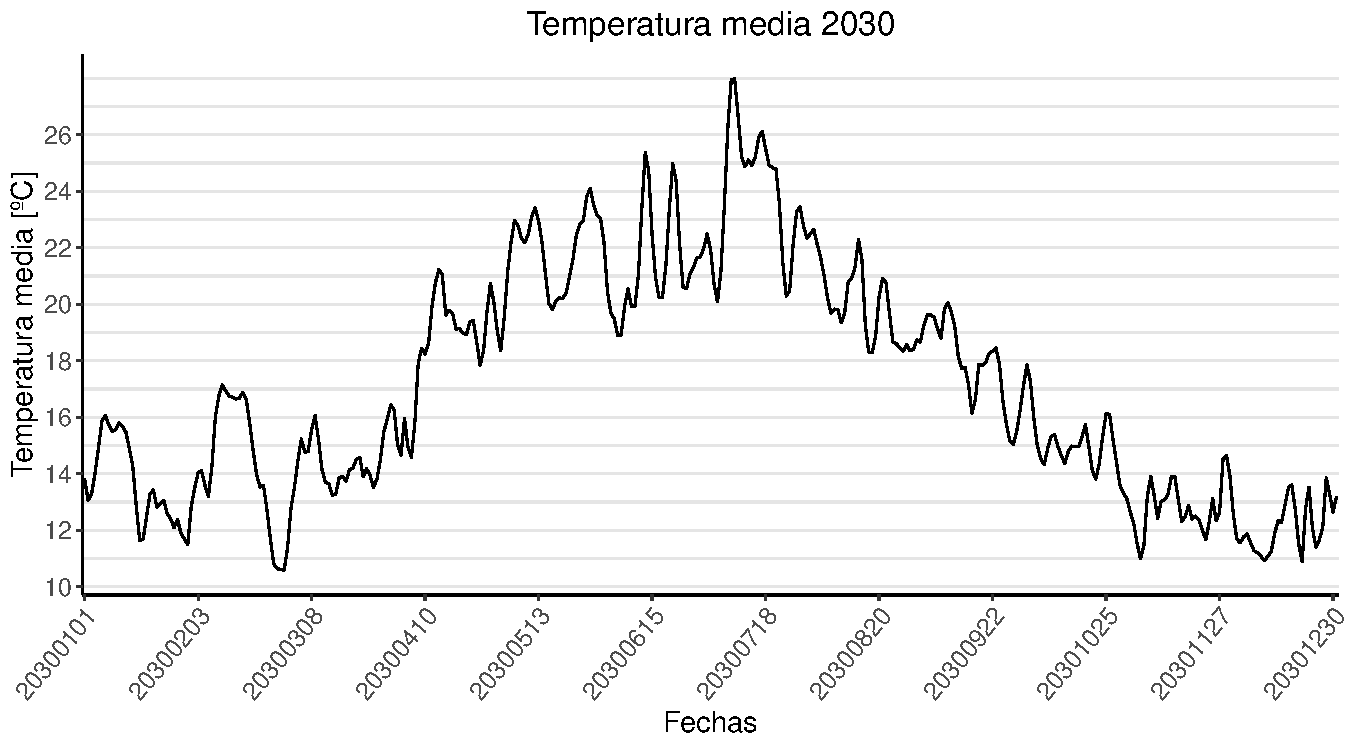
\includegraphics[width=\textwidth]{fotos/plot4.pdf}
\end{subfigure}
\hfill
\begin{subfigure}{0.415\textwidth}
\centering
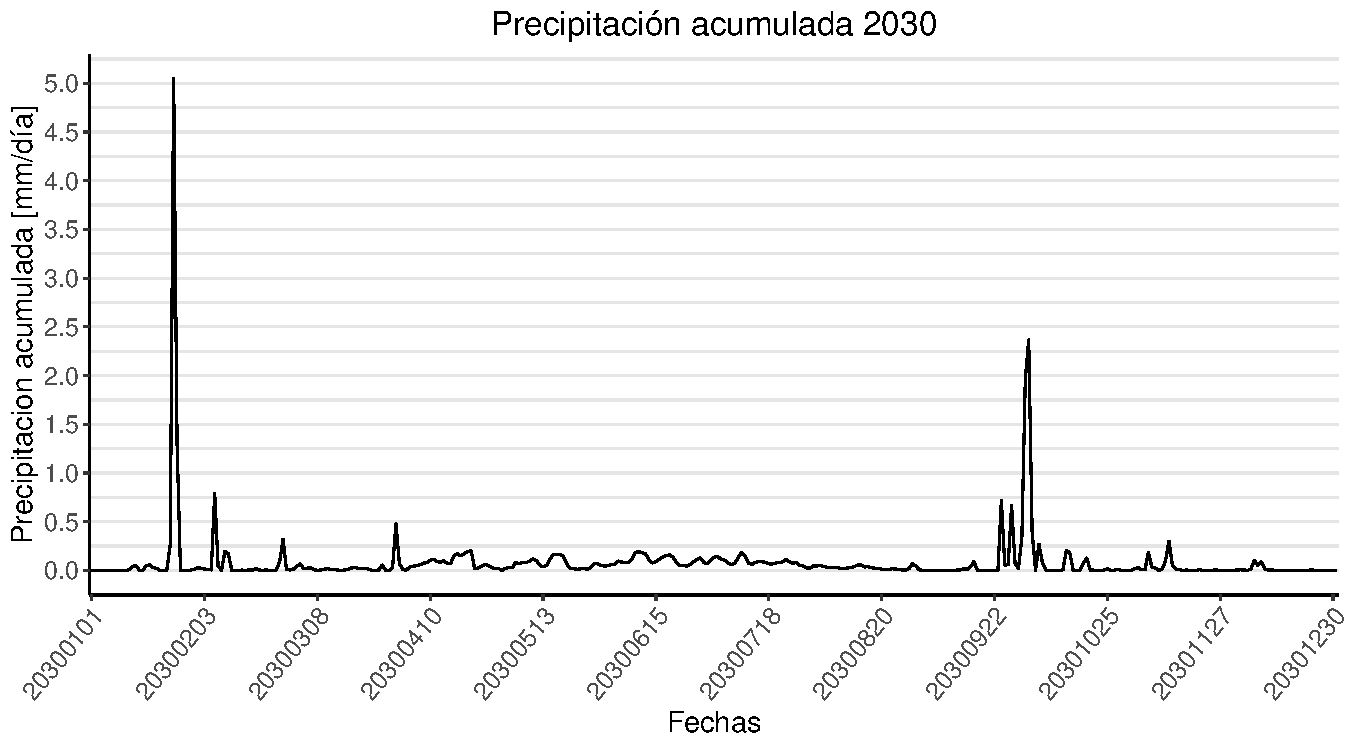
\includegraphics[width=\textwidth]{fotos/plot9.pdf}
\end{subfigure}
\caption{Variabilidad diaria de la temperatura media y la precipitación acumulada en 2030.}
\label{fig:1}
\end{figure}

En la figura \ref{fig:1} se muestra la variabilidad diaria de ambas magnitudes. En el caso de la temperatura se tiene un resultado familiar, que muestra un aumento de temperatura desde primavera hasta agosto, cuando remite suavemente hasta ya entrado el otoño. Para el caso de la precipitación acumulada, se muestra un patrón de escasa lluvia, a excepción de picos puntuales que superan en más del 500\% lo esperado (algunos en más de un 1000\%).

\subsection{Distribución espacial}

Para visualizar la distribución espacial de las variables, se mostrarán dos gráficos con la misma información, pero que permiten estudiarla de forma distinta. Un gráfico de cajas permite ver con claridad la variabilidad de las magnitudes en las tres series temporales escogidas, mientras que un mapa de calor permite asociar esta variabilidad con cada zona geográfica. 

\begin{figure}[H]
\centering
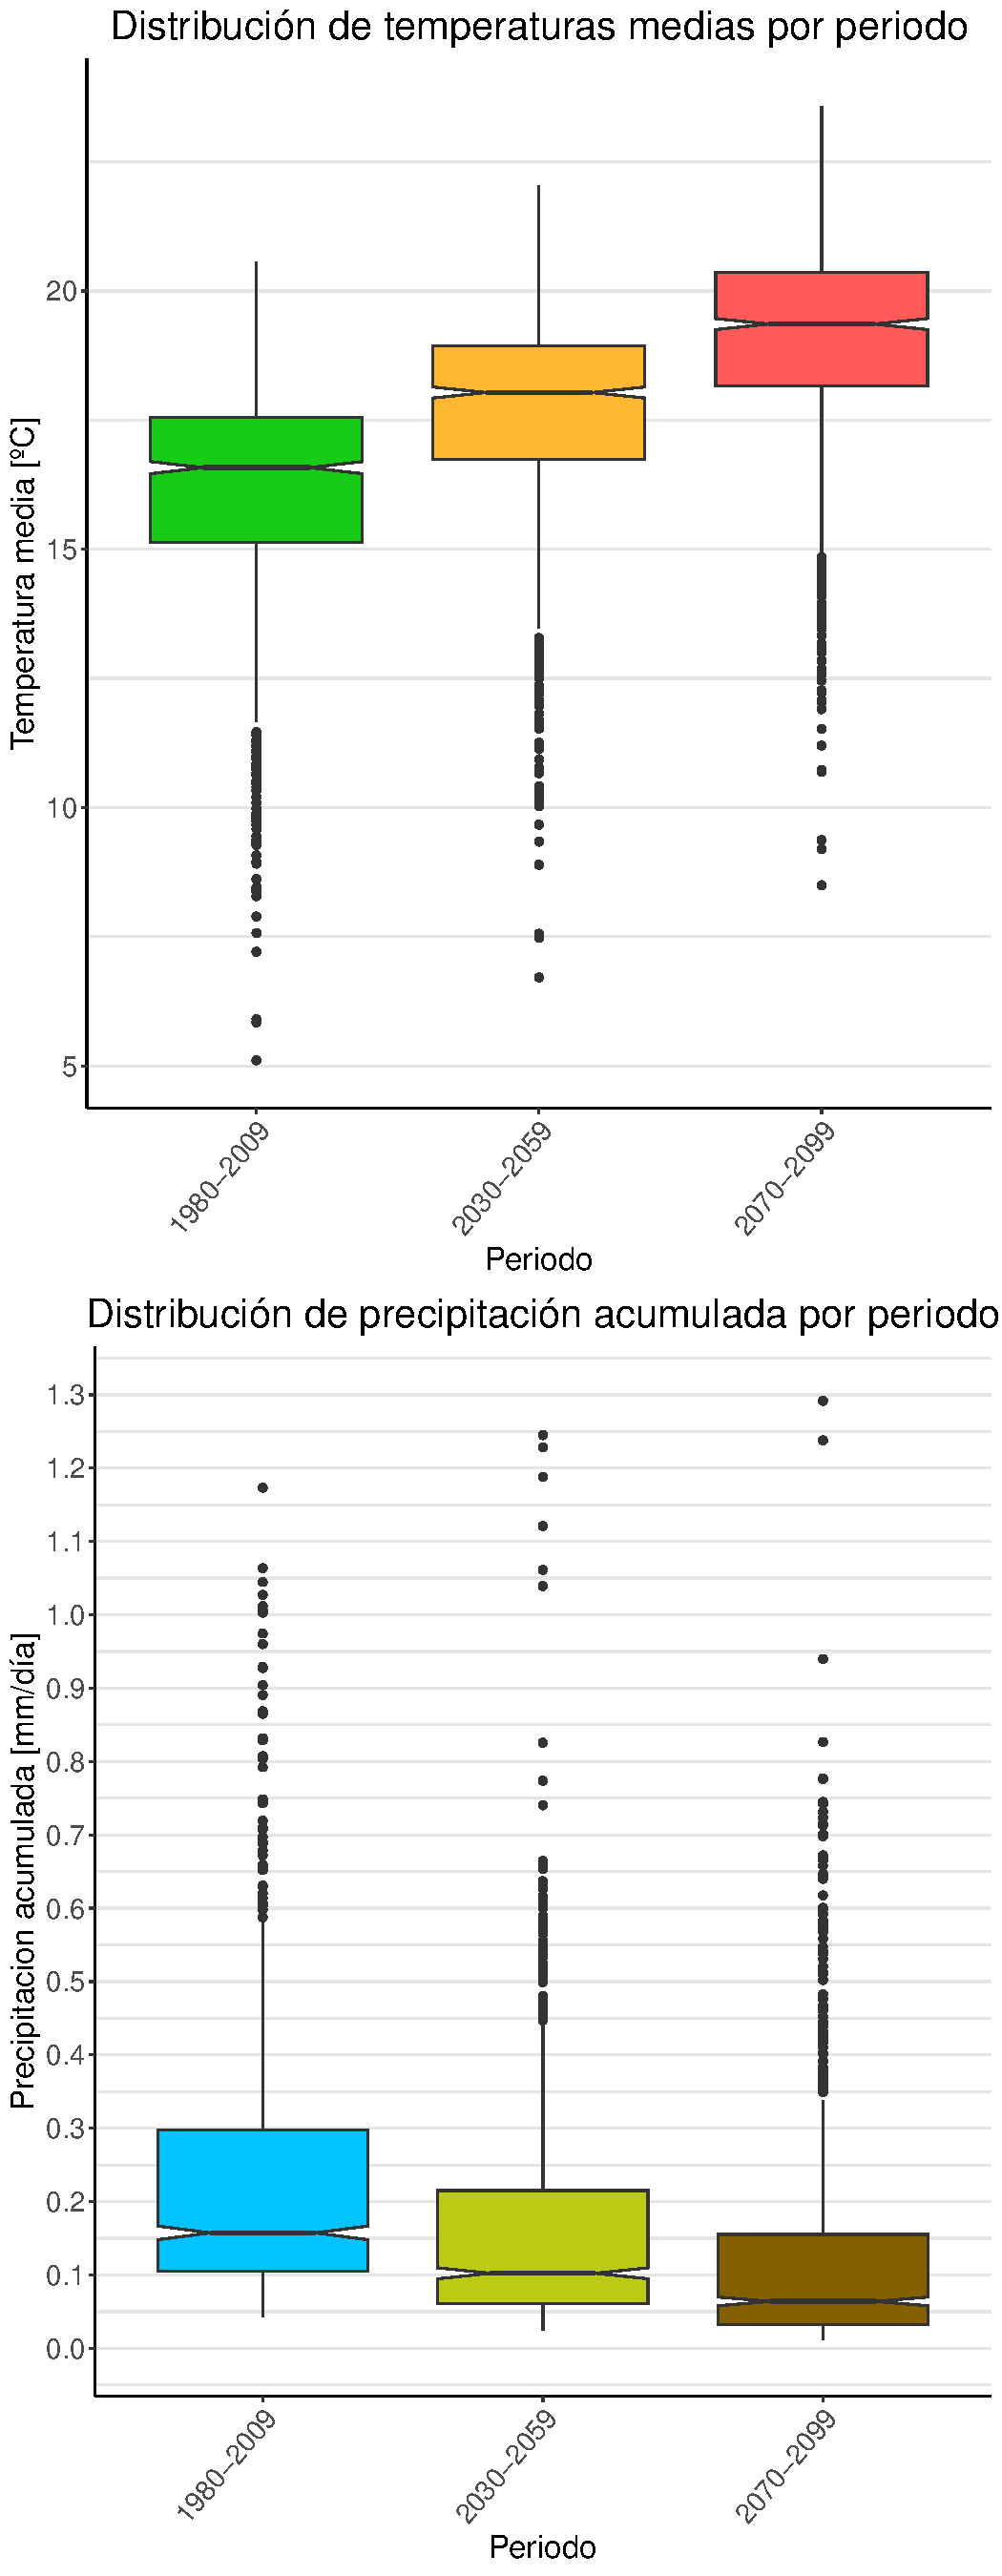
\includegraphics[width=0.345\textwidth]{fotos/plot_esp.pdf}
\caption{Distribución espacial de las variables en cada serie temporal.}
\label{fig:3}
\end{figure}

En la figura \ref{fig:3} se hace evidente el aumento de la temperatura media que se tenía como objetivo para este trabajo, así como el descenso en la precipitación acumulada de aquí a final de siglo. Cabe destacar que los \textit{outliers} en la temperatura corresponden simplemente a las zonas más elevadas de las islas, mientras que en la precipitación acumulada se corresponden con las zonas más lluviosas (ambas suelen coincidir, y son de escasa extensión territorial). Esto se ve con más claridad en la figura \ref{fig:4}, donde se aprecia cómo estas zonas son cada vez de menor tamaño.

\section{Inferencia}

Si bien se ha visto visualmente lo que se quería demostrar, se puede hacer un análisis inferencial para confirmar los resultados. Se evaluarán tanto intervalos de confianza como contrastes de hipótesis para ratificar la diferencia significativa entre las medias de las variables en los periodos temporales escogidos con ambos métodos. En este caso, se usarán únicamente el periodo pasado (1980-2009) y el futuro lejano (2070-2099).

\subsection{Intervalos de confianza}

Se evaluarán los intervalos de confianza al 95\% en busca de solapamiento (tabla \ref{tb:3}). Al no solaparse, se confirma un cambio significativo en ambas variables. Concretamente, un aumento de temperaturas medias de unos $3^\circ$ y un descenso de las precipitaciones acumuladas en poco más del $20\%$.

\begin{table}[H]
\centering
\resizebox{0.33\textwidth}{!}{
\begin{tabular}{ccc}
\hline
\textbf{Periodo} & \textbf{Intervalo $[^\circ C]$} & \textbf{Intervalo [mm/día]} \\ \hline
1980-2009 & $[15.88, 16.17]$ & $[0.22, 0.24]$ \\ \hline
2070-2099 & $[18.88, 19.14]$ & $[0.13, 0.16]$ \\ \hline
\end{tabular}
}
\caption{Salida de código: intervalos de confianza al 95\% para temperatura y precipitación.}
\label{tb:3}
\end{table}

\subsection{Contraste de hipótesis}

Se realizará el mismo contraste para ambas variables. Se tomará como hipótesis nula la igualdad de las medias en ambos periodos temporales, y como hipótesis alternativa la no igualdad, fijando la significancia al 5\%. 

\begin{equation}
\begin{matrix}
H_0: & \mu_{1980-2009} = \mu_{2070-2099} & \\
H_1: & \mu_{1980-2009} \neq \mu_{2070-2099} &
\end{matrix}
\end{equation}

Para temperatura se tiene un p-valor de $2.11 \cdot 10^{-168}$, mientras que para las precipitaciones se obtiene un p valor de $2.50 \cdot 10^{-20}$. En ambos casos, al ser el valor menor de $0.05$, se rechaza la hipótesis nula y se confirma la no igualdad de las medias de las variables en el pasado y el futuro lejano.

\section{Conclusiones}

Se quería probar el aumento significativo de la temperatura media y el descenso de la precipitación acumulada en las Islas Canarias haciendo uso de predicciones de modelos neuronales. Este proceso es un poco complicado con una visualización numérica, pero una representación visual adecuada de los datos lo facilita en gran medida. \\

Estos se comprobaron también usando técnicas de inferencia, lo cual da un resultado analítico: a partir del no solapamiento de los intervalos de confianza se concluyó una diferencia significativa, y con un contraste se demostró analíticamente la no igualdad de las medias de ambas variables bajo estudio. 

\addtocounter{figure}{-3}
\begin{figure*}
\centering
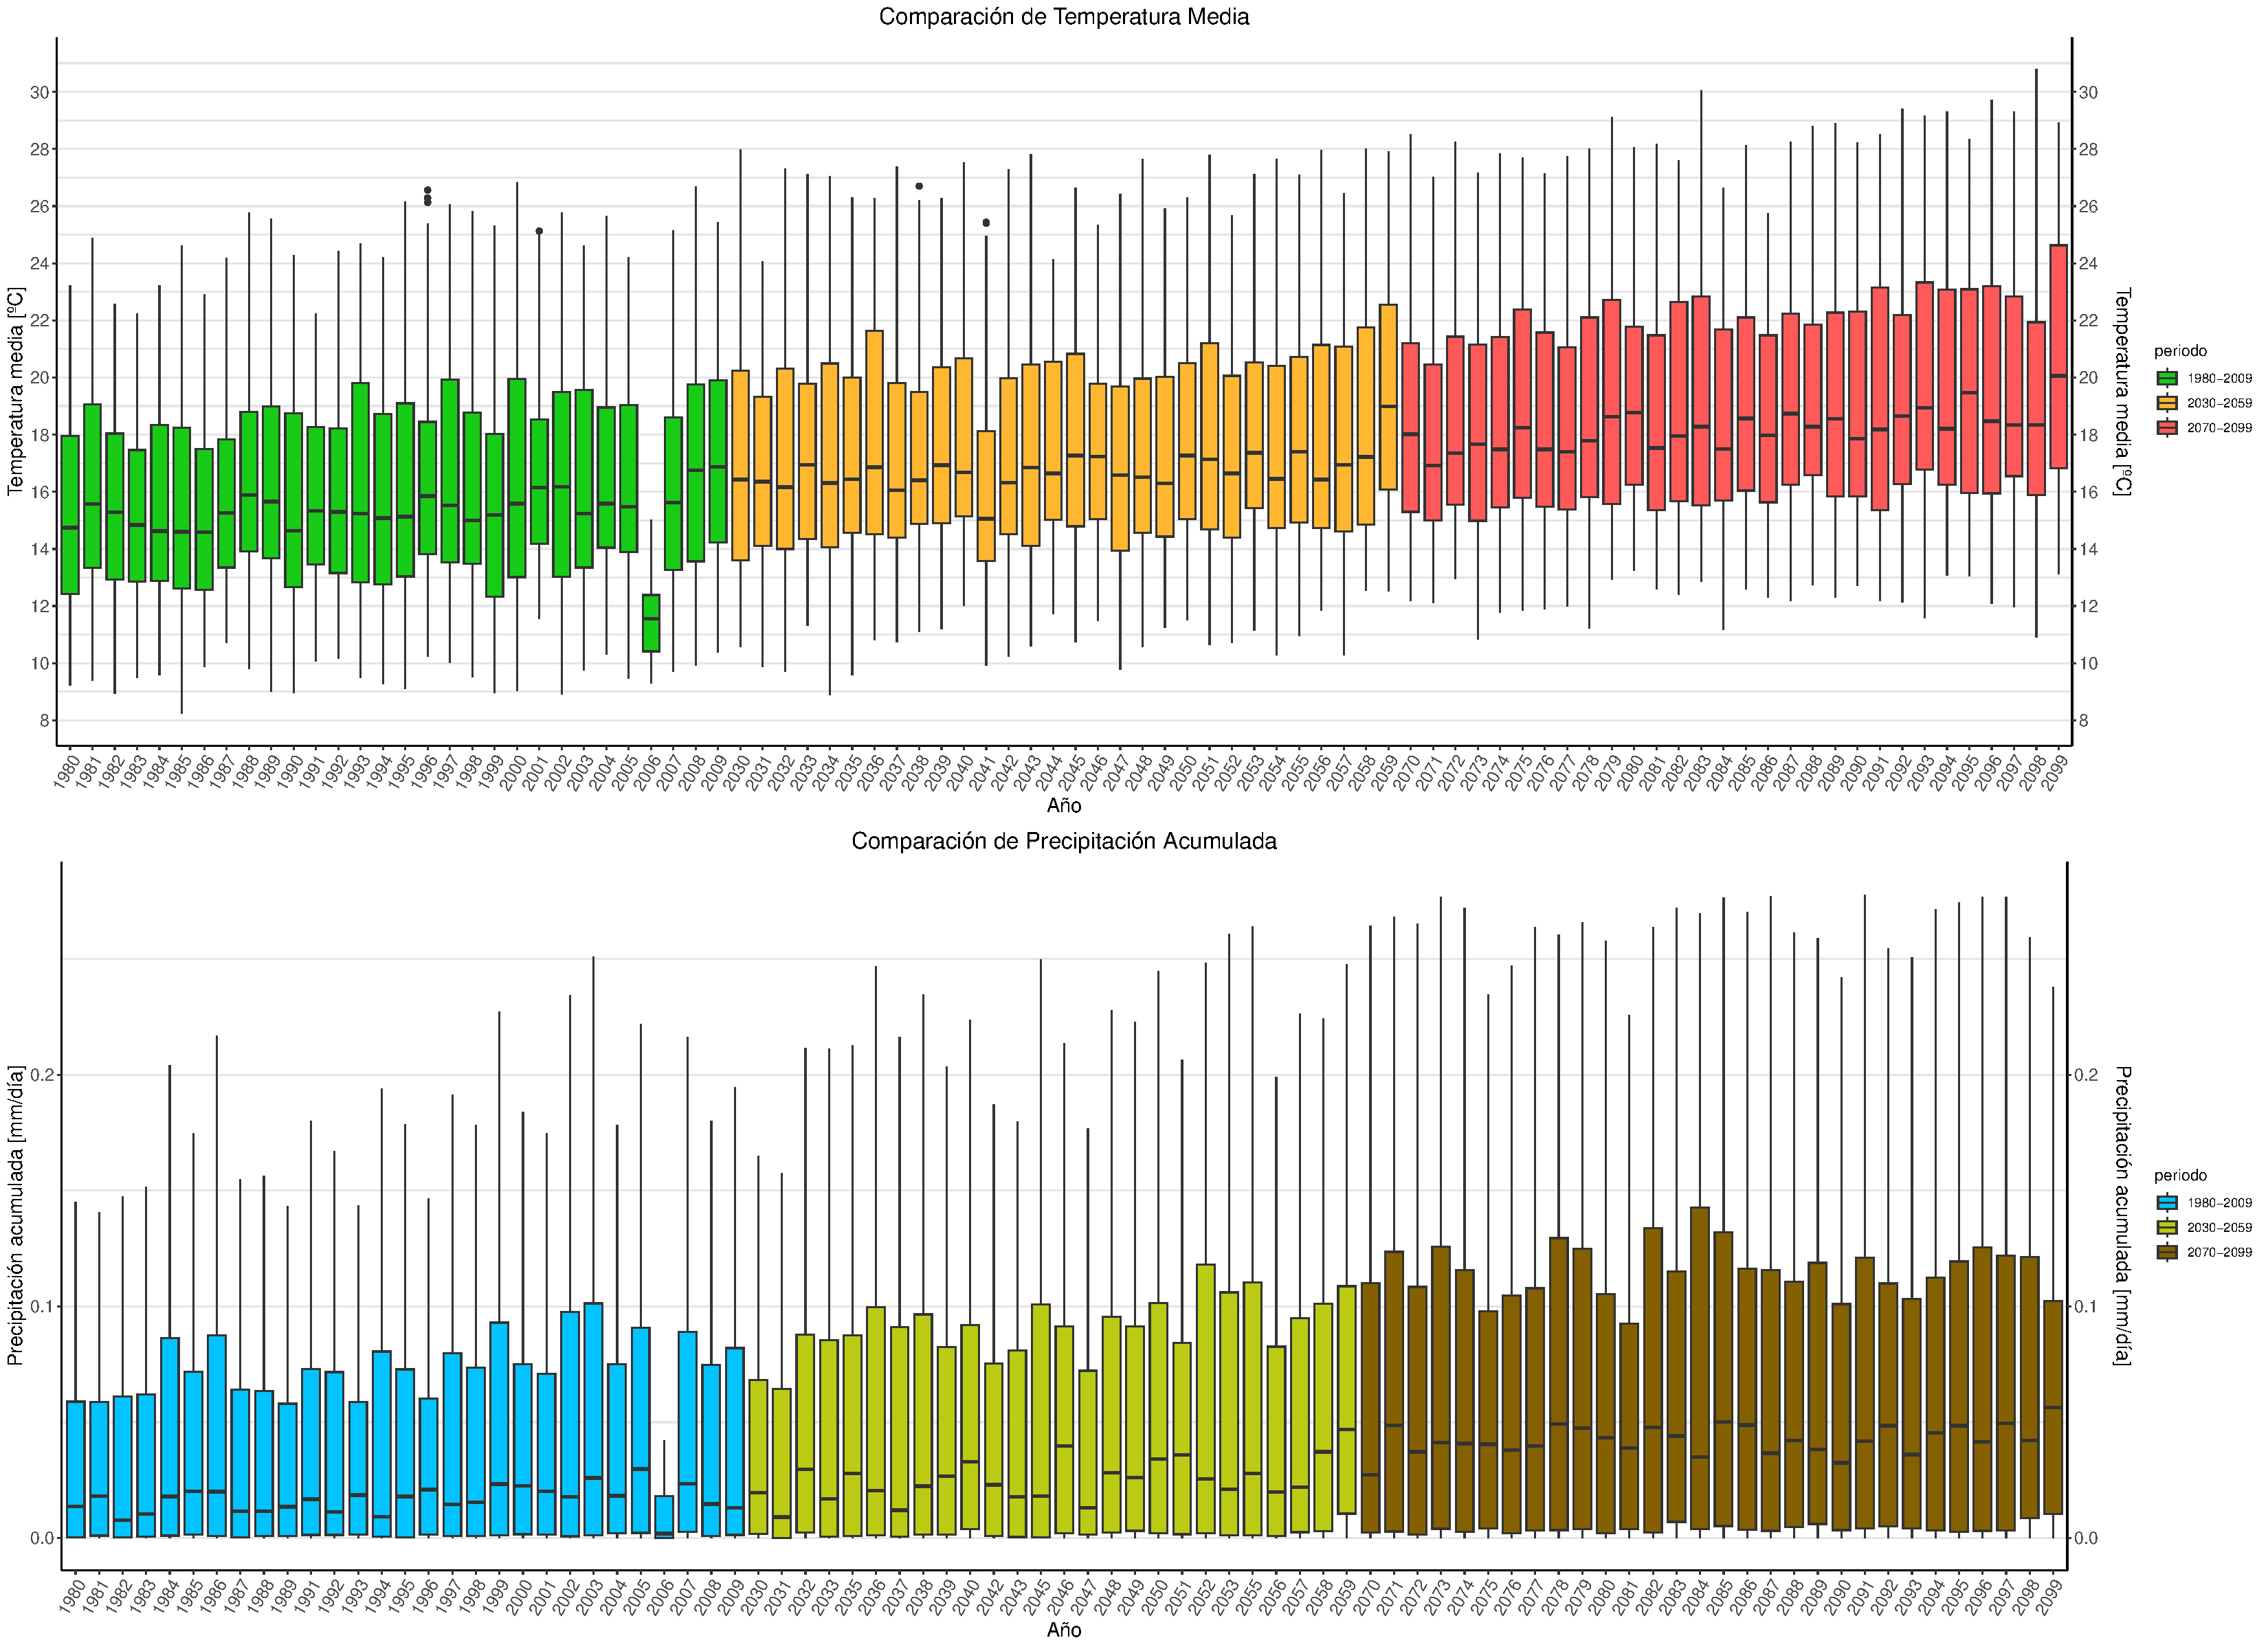
\includegraphics[height=0.7\textheight, angle=270]{fotos/combined_plot.pdf}
\caption{Variabilidad temporal de la temperatura media y la precipitación acumulada desde 1980 hasta 2099.}
\label{fig:2}
\end{figure*}

\addtocounter{figure}{2}
\begin{figure*}
\centering
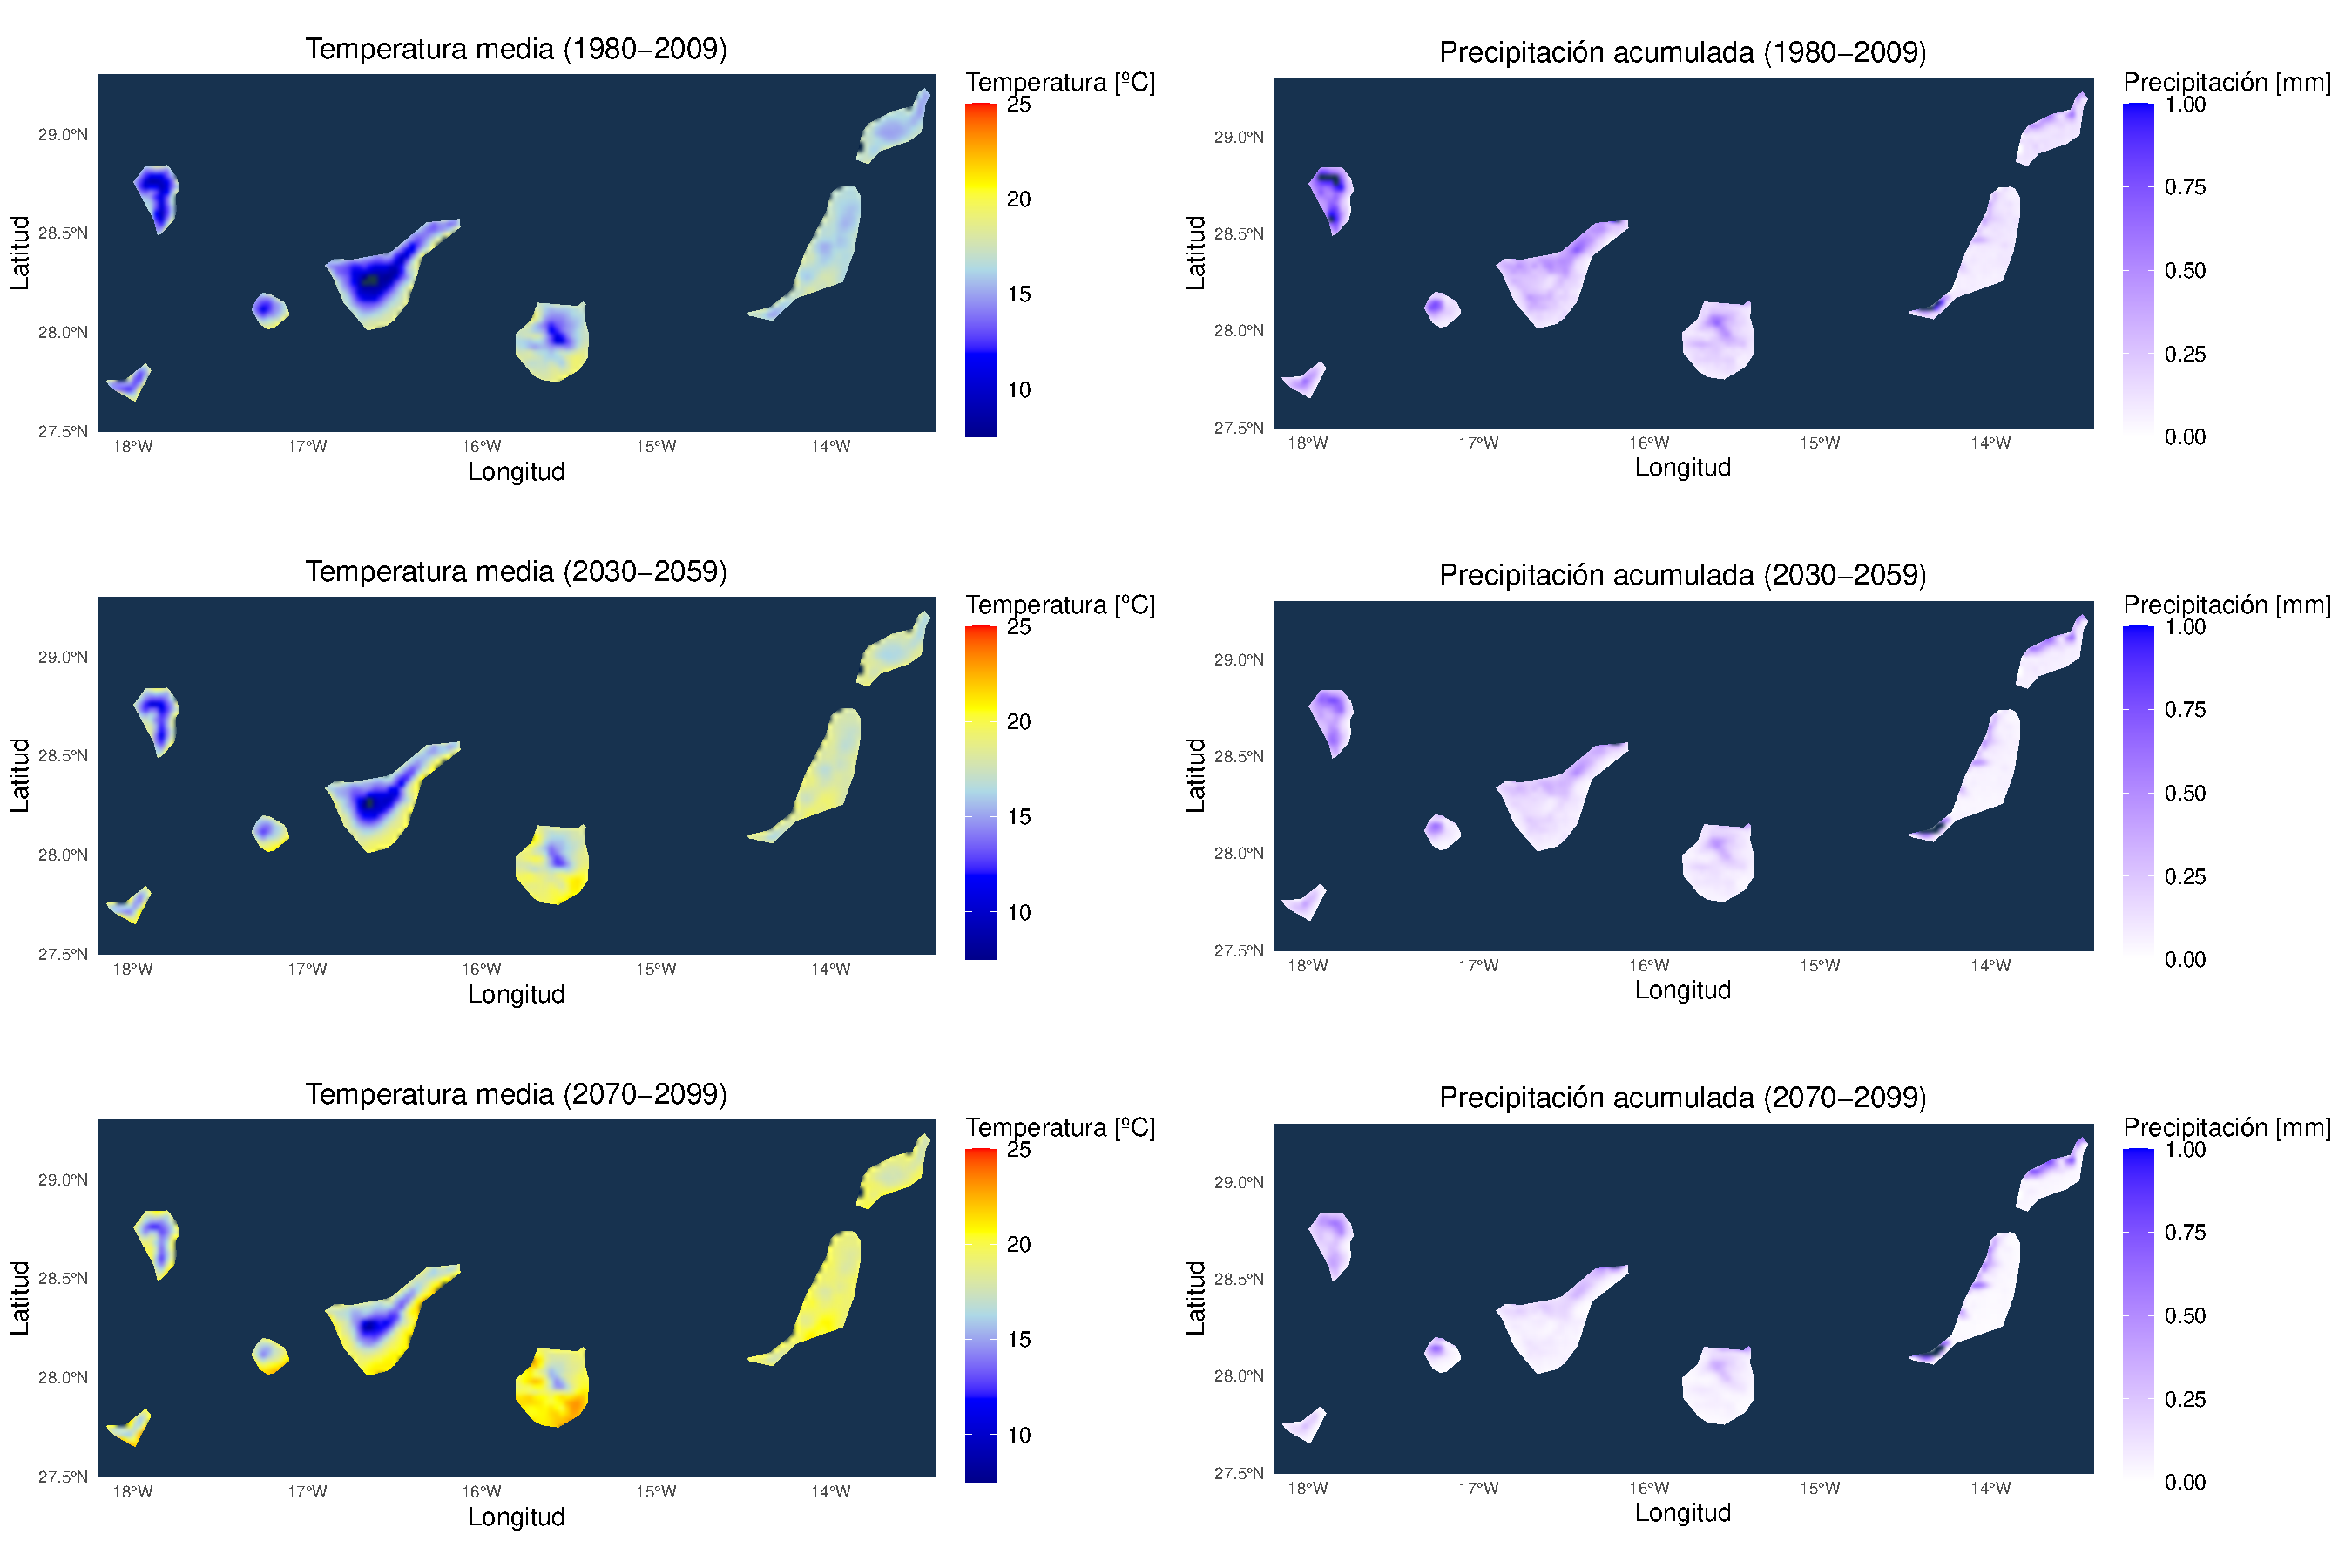
\includegraphics[width=\textwidth]{fotos/map_esp.pdf}
\caption{Distribución espacial de las variables en cada serie temporal.}
\label{fig:4}
\end{figure*}


\end{document}
